\documentclass[12pt,a4paper]{article}
\usepackage[cm]{fullpage}
\usepackage[utf8]{inputenc}
\usepackage{indentfirst}
\usepackage{wrapfig}
\usepackage{placeins}

\usepackage{graphicx}
\graphicspath{ {./img/} }


\usepackage[hidelinks]{hyperref}
\usepackage{float}

\usepackage{listings}
\usepackage{color}

\let\oldsection\section
\renewcommand\section{\clearpage\oldsection}

\newcommand{\dofigure}[3][H]{
    \begin{figure}[#1]
        \centering
        \includegraphics[width=\textwidth]{#2}
        \caption{#3}
    \end{figure}
}

\newcommand{\chip}[1]{{\itshape#1}}
\newcommand{\pin}[1]{\textbf{#1}}

\newenvironment{pins}{
    
    \let\oldpin\pin
    \renewcommand{\pin}[1]{\item\oldpin{##1}}
    \newcommand{\inputs}[1]{
        
    Input pins:\begin{itemize}##1\end{itemize}}
    \newcommand{\outputs}[1]{
        
    Output pins:\begin{itemize}##1\end{itemize}}
}{}

\makeatletter 
\def\WFfill{\par 
    \ifx\parshape\WF@fudgeparshape 
    \nobreak 
    \ifnum\c@WF@wrappedlines>\@ne 
    \advance\c@WF@wrappedlines\m@ne 
    \vskip\c@WF@wrappedlines\baselineskip 
    \global\c@WF@wrappedlines\z@ 
    \fi 
    \allowbreak 
    \WF@finale 
    \fi 
} 
\makeatother

\begin{document}
    \begin{titlepage}
        \begin{center}
            \vspace*{0.3\textheight}

            {\Huge \textbf {Enhanced Pong}}

            {\LARGE Digital platforms project B}

            \vspace{1.5cm}
            Merzlyakov Ilya, Batenko Nikita, Feshchenko Igor

            \vfill
            Novosibirsk State University \\
            2021

        \end{center}
    \end{titlepage}
    \tableofcontents


    \section{Overview}
    \dofigure{main}{Game display}
    We implemented a fully functional Pong (or TV-Tennis) game, based on design document, but with some extensions:\begin{itemize}
        \item now, ball can fly at 512 different angles (compared to 4 from original specification)
        \item when one player gets a point, the ball respawns at the side of hit player directed to other player
        \item game is not endless now, it ends when one player gets 5 points
        \item animations: they play on system start and after game over 
        \item real gamepad is used, to support it logisim library was written in Kotlin 
        \item ball velocity is slightly changed in the middle of the screen, so AI will miss sometimes
        \item ball direction changes based on which part of the bat it was reflected by
        \item ball velocity always equals to 1
    \end{itemize}


    \section{Hardware design}
    \dofigure{scheme.png}{Hardware architecture}
    Or project's circuit can be divided into three subsystems:
    \begin{itemize}
        \item video system - draws gameplay elements (ball and bats) and plays animations;
        \item gameplay system (\chip{kinematic controller}) - responsible for actual gameplay;
        \item ai system - controls bot movement.
    \end{itemize}
    Also there is \chip{main} chip, which glues all these systems together and also contains graphical display.
    Now all said systems will be described.

    

    \subsection{Video system}
    This system is responsible for rendering graphics on 32x32 display. It can operate in two modes: {\itshape gameplay} mode and {\itshape video} mode. These mode are selected with \pin{enable} pin of \chip{video\_player} chip. In the first mode, ball and bats are visible on the screen; in the second mode, \chip{video\_player} can draw arbitrary images on screen. This subsection consists of the following chips: 
    \chip{video\_chip}, \chip{video\_section} and \chip{video\_player}.

    \subsubsection{Video\_chip}
    \dofigure{video_chip}{Video\_chip}
    This chip controls one column of the screen; to control display we need to connect 32 of these chips in a row. Because this chip is intended to be connected to other \chip{video\_chip}s, most of it's inputs are wired directly to corresponding outputs (except \pin{chipID}). \pin{chipID} actually defines column number the chip is connected to, so \pin{chipID out} pin is set to \pin{chipID input}+1.
    In {\itshape gameplay} mode this chip draws ball at specified height, if \pin{ballX}  equals to \pin{chipID}. Also it draws bat, if \pin{chipID} equals to 3 (left bat) or 28 (right bat). \pin{leftbatY} and \pin{rightbatY} define Y coordinate of the bottommost pixel of corresponding bat. The {\itshape video} mode is enabled by bit 7 of \pin{controlIn} and will be described later.

    \subsubsection{Video\_section chip}
    This is just an assembly of 8 \chip{video\_chip}s connected one after another. 

    \subsubsection{Video\_player}
    \dofigure{video_player}{Video\_player chip}
    \begin{pins}
        \inputs{
            \pin{enable} - If 1, video mode is active
            \pin {num} - Animation number
            \pin {set} - When 1, starts animation with specified number
            \pin {clock} 
        }

        \outputs{
            \pin {ctrl} - \chip{video\_chip} control
            \pin {data} - Current pixel column
        }
    \end{pins}

    This chip has ROM with all animations. One animation is simply a sequence of frames, and one frame is a sequence of 32 32-bit values (columns). To draw one frame of animation, this chip must send all columns of this frames to corresponding \chip{video\_chip}s. To do so, it firstly selects needed chip with bits 0-4 of \pin{ctrl}. Then it sets \pin{data} to current column of the image, and by rising bit 5 of \pin{ctrl} it tells selected \chip{video\_chip} to store column data in intermediate register. When the whole frame is stored in these registers, it raises bit 6 of \pin{ctrl}, so all \chip{video\_chip}s update their outputs simultaneously. Bit 7 of \pin{ctrl} switches \chip{video\_chip}s into {\itshape{video}} mode.

    Constants below the chip define start and end addresses of all animations.


    \subsection{AI}
    \dofigure{ai}{AI chip}
    \begin{pins}
        \inputs{
            \pin{bx} - X coordinate of ball
            \pin{by} - Y coordinate of ball
            \pin{vx} - X component of velocity
            \pin{vy} - Y component of velocity
            \pin{reset} - Cdm-8 reset
            \pin{clock}
        }
        \outputs{
            \pin{result} - Calculated bat position
        }
    \end{pins}

    To predict ball position, Cdm-8 must perform multiplication and division.
    Since ball coordinates and velocity are represented as 16-bit fixed-point numbers (fraction part stored in bits 0-6), Cdm-8 is not powerful enough to perform multiplication and division, so hardware multiplier and divider are mapped to it's memory to speed up calculations.

    Cdm-8 here is used in Von Neumann mode (code and data are in the same address space), but it reads program from ROM mapped to a lower half of address space, and uses RAM mapped to a higher half of address space, so there is no need for loading firmware into RAM on every system start.

    


    \subsection{Kinematic controller}
    \dofigure{kinematic_overview}{Kinematic controller overview}
    \begin{pins}
        \inputs{
            \pin{reset} - game restart
            \pin{ly} - left bat position
            \pin{ry} - right bat position
        }
        \outputs{
            \pin{xb} - 16-bit X coordinate of ball
            \pin{yb} - 16-bit Y coordinate of ball
            \pin{vx} - 16-bit X component of ball velocity
            \pin{vy} - 16-bit Y component of ball velocity
            \pin{a} - left player score
            \pin{b} - right player score
            \pin{five pins on east side} - output to \chip{video\_chip}s
        }
    \end{pins}
    This chip is responsible for all gameplay mechanics.

    Let's define some internal terminology for later use in this subsection:\begin{itemize}
        \item hit - event triggered when ball touches vertical edge of the screen
        \item posReset - event triggered on game reset and hit
        \item bx, by - ball coordinates
        \item vx, vy - ball velocity
    \end{itemize}
    Ball coordinates and velocity are represented as 16-bit fixed-point numbers (fraction part stored in bits 0-6).


    Every clock cycle  ball coordinates are updated by corresponding velocity components, then velocity is updated, if ball collision occurred. Also it counts players' score and adds smoothness to right bat's movement (since AI sets it's position only once, while the ball is moving towards it). Bat collision is detected by comparison of x coordinate of ball and bar, and wall collision is detected, when addition of velocity component to ball coordinate causes overflow.
    
    

    Now some parts of kinematic controller will be described with more detail.
    \subsubsection{Ball position calculation}
    \begin{wrapfigure}{rh}{0.5\textwidth}
        \centering
        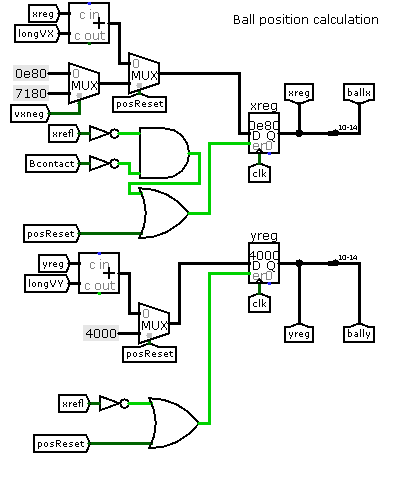
\includegraphics[width=0.48\textwidth]{ball_position_calculation}
        \caption{Ball position calculation unit}
    \end{wrapfigure}
    This part of \chip{kinematic} controller is responsible for storing and updating (on every clock cycle) ball coordinates. If there was no hit, it calculates $bx \leftarrow bx+vx$ and $by \leftarrow by+vy$. If there was a hit, it resets ball position and places the ball on side of the screen, so the ball will fly through the whole screen to player who got a point at this tick (side is selected based on the ball direction).
    \WFfill
    \WFclear

    \subsection{Ball velocity calculation}
    \dofigure{ball_velocity_calculation}{Ball velocity calculation unit}
    This part is responsible for storing and updating of ball velocity.
    It separately stores ball angle (a value from $[-52^{\circ};+52^{\circ}]$ mapped to $[-127;127]$) and ball direction along X axis (in vxneg register, 1 - negative direction, 0 - positive direction). If posReset happens, it sets angle to random value, and sets X direction and the ball will fly towards the player who got point on this tick. If the ball collides with the bat, it changes X direction to opposite.
    When ball hits horizontal edge of the screen, it just negates it's angle, but when the ball is reflected by bat, it sets angle to $by-bat$. For example, if the ball was reflected by top side of the bat, it will fly upwards.

    Also this unit slightly changes angle by random value after the ball travels half a distance from left side to right side of the screen, so AI will miss sometimes.

    Vx and vy are calculated as $\cos{angle}$ and $\sin{angle}$ respectively by \chip{velocity\_calculator} chip. It just reads this values from pregenerated ROM chips.

    $52^{\circ}$ is the maximum angle that does not cause overflow when calculating $(228-bx)*\tan{angle}$
    




    
    \subsection{Miscellaneous circuitry}
    \dofigure{misc}{Miscelanious circuitry}
    \chip{AI} chip is placed in the top right corner of the picture. Note that bx, by, vx, vy are connected to it through registers. Their values are updated only when ball starts flying from left  to right. These registers serve two purposes: first, they prevent ai from cheating by setting bat coordinate to ball coordinate in loop, and second, they prevent data corruption, since Cdm-8 cannot read input values instantly, and these values can change in the middle of reading.

    \chip{Video\_chip} is placed in the bottom right corner. It is connected to animation selection circuitry. Animation numbers: 0 - startup, 1 - win, 2 - loose.


    \section{Cdm-8 software}
    To predict ball position when it's x coordinate will be equal to 228 (coordinate of right bat), Cdm-8 must calculate following formula: {\Large $result=by + {(228-bx)*vy \over vx}$}. Here is complete and well-commented source code for Cdm-8. It's flowchart is attached below.

    \definecolor{eclipseBlue}{RGB}{42,0.0,255}
    \definecolor{eclipseGreen}{RGB}{63,127,95}
    \lstset{
        breakatwhitespace=true,
        breaklines=true,
        numbers=left
    }
    \lstdefinelanguage{cdm8}{
        morecomment=[l]{\#},
        commentstyle=\color{eclipseGreen},
        keywordstyle=\color{eclipseBlue},
        morekeywords={r0, r1, r2, r3, ext, ld, st, ldi, ldc, move, add, addc, sub, cmp, and, or, xor, not, neg, dec, inc, shr, shra, shla, rol, push, pop, jsr, rts, osi, osix, rti, crc, br, beq, bz, bne, bnz, bhs, bcs, blo, bcc, bmi, bpl, bvs, bvc, bhi, bls, bge, blt, bgt, ble, ret, nop, wait, halt, pushall, popall, setsp, addsp, ldsa, ioiosix, rti, asect, rsect, end, dc, ds, tplate, p0, p1, p2, p3, p4, p5, p6, p7, run, else, if, fi, is, gt, lt, le, ge, mi, pl, eq, ne, z, nz, cs, cc, vs, vchi, lo, hs, ls, macro, mpop, mpush, mend, continue, wend, until, while, save, restore, define, stsp, ldsp, stays, true, break, tst, clr, do, then, unique, first_item, item, last_item, jmp, jsrr, shl, banything, bngt, bnge, bneq, bnne, bnlt, bnle, bnhi, bnhs, bncs, bnlo, bnls, bncc, bnmi, bnpl, bnfalse, bntrue, bnvs, bnvc, bnvs, define, ldv, stv, ei, di}
    }
    \lstinputlisting[language=cdm8]{../ai.asm}

    \begin{figure}[H]
        \centering
        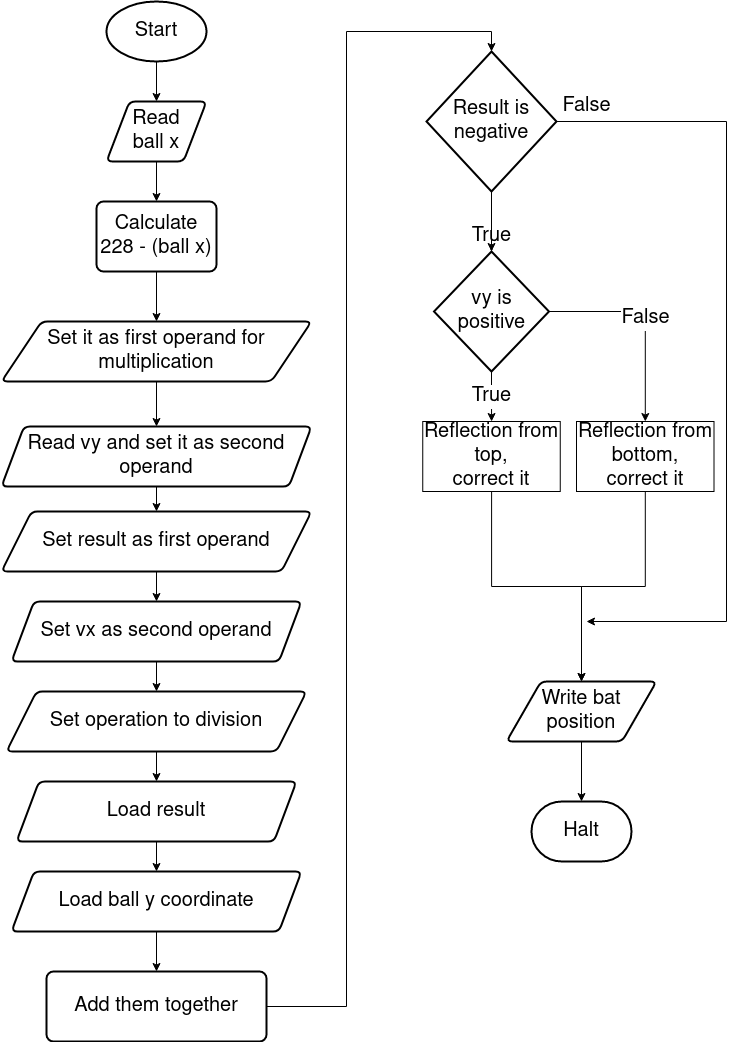
\includegraphics[height=0.9\textheight]{flowchart.png}
        \caption{Algorithm flowchart}
    \end{figure}

    \section{Software}
    To make development process easier, and to add more features to the project, some software was developed.
    \subsection{generate\_firmwares.py script}
    This script was written to automatically generate 4 binary images:\begin{itemize}
        \item ai.img - compiled Cdm-8 program, this script uses cocas.py from CocoIDE distribution to do it.
        \item animation.img - all animations generated by this script. Used in \chip{video\_player}
        \item cos.img and sin.img - tables for \chip{velocity\_calculator} chip
    \end{itemize}
    This script is pretty well commented and will not be described here.
    \subsection{AutoRAM Logisim library}
    It is named AutoRAM due to historical reasons (it was used to automatically load Cdm-8 firmware to RAM on simulation reset).
    Now it is used to access real gamepad connected to host logisim runs on.
    This library is written in kotlin, it's sources are available at github: {\color{blue}\url{https://github.com/leadpogrommer/logisim_convinient_ram}} (yes, I know about a typo in repository name)



\end{document}